\documentclass[oneside,a4paper,14pt]{extarticle}

\usepackage[russian]{babel}
\usepackage{fontspec}
\setmainfont{Times New Roman}
\setmonofont{Courier New}
\usepackage[a4paper,top=2cm,bottom=2cm,left=2.5cm,right=1.5cm]{geometry}
\usepackage{textcomp}
\usepackage{indentfirst}
\usepackage{minted}
\usepackage{xcolor}
\usepackage{enumitem}
\usepackage{caption}
\usepackage{amsmath}
\usepackage{float}
\usepackage{graphicx}
\usepackage{titlesec}
\usepackage{hyperref}

\titleformat{\section}{\normalsize\bfseries}{\thesection}{1em}{}
\titleformat{\subsection}{\normalsize\bfseries}{\thesubsection}{1em}{}

\renewcommand\baselinestretch{1.33}\normalsize
\setlength{\parindent}{1.25cm}

\renewcommand{\listingscaption}{Листинг}
\setminted[python]{
	fontsize=\footnotesize,
	linenos,
	frame=single,
	breaklines,
	autogobble,
	baselinestretch=1
}
\setlength{\emergencystretch}{2em}

\begin{document}

\newpage
\thispagestyle{empty}
\begin{center}
	МИНИСТЕРСТВО НАУКИ И ВЫСШЕГО ОБРАЗОВАНИЯ\\
	РОССИЙСКОЙ ФЕДЕРАЦИИ
	ФЕДЕРАЛЬНОЕ ГОСУДАРСТВЕННОЕ БЮДЖЕТНОЕ\\
	ОБРАЗОВАТЕЛЬНОЕ
	УЧРЕЖДЕНИЕ ВЫСШЕГО ОБРАЗОВАНИЯ\\
	«ВЯТСКИЙ ГОСУДАРСТВЕННЫЙ УНИВЕРСИТЕТ»\\
	Институт математики и информационных систем\\
	Факультет автоматики и вычислительной техники\\
	Кафедра электронных вычислительных машин
\end{center}

\vspace{20mm}

\begin{center}
	Отчёт по лабораторной работе №7\\
	по дисциплине\\
	<<Программирование>>
\end{center}

\vspace{48mm}

\noindent
Выполнил студент гр. ИВТб-1303-06-00 \hfill \rule[-0,5mm]{30mm}{0.15mm}\,/Шубин В. Ю./
\newline
Проверил преподаватель кафедры ЭВМ \hfill \rule[-0,5mm]{30mm}{0.15mm}\,/Баташев П.А./

\vfill

\begin{center}
	Киров\\
	2026
\end{center}

\newpage
\thispagestyle{empty}

\section{Цель и задачи работы}

Цель работы: освоение практических навыков создания интерактивных дашбордов в Python, включая интеграцию pandas DataFrame с графическими библиотеками matplotlib и seaborn, встраивание графиков в окно Tkinter через бэкенд FigureCanvasTkAgg, реализацию событийно-ориентированной архитектуры (callbacks, event loop), динамическую фильтрацию, агрегацию и feature engineering «на лету», а также проектирование устойчивого процедурного кода без использования классов.

Задачи:
\begin{enumerate}[leftmargin=*]
	\item Сформировать и подготовить набор данных с категорийными и временными признаками.
	\item Реализовать предобработку данных: очистку выбросов, клаппинг физических величин, расчёт скользящих средних и производных признаков.
	\item Интегрировать графический движок Matplotlib/Seaborn с GUI Tkinter через адаптер FigureCanvasTkAgg.
	\item Разработать панель управления с интерактивными элементами (выпадающие списки, переключатели агрегации, кнопки смены типа графика).
	\item Реализовать механизм безопасного обновления данных через \texttt{.copy()} и перерисовки через \texttt{canvas.draw\_idle()} без блокировки основного потока.
	\item Внедрить экспорт визуализаций в PNG/PDF.
\end{enumerate}

\section{Описание варианта}

Вариант №8: GPS телеметрия транспорта.

Предметная область: мониторинг автопарка. Данные телеметрии фиксируют скорость, уровень топлива, обороты двигателя и статус ускорения для каждого автомобиля; анализ позволяет оценить стиль вождения, состояние датчиков и распределение нагрузки по транспортным средствам.

Основные метрики (поля датасета):
\begin{itemize}[leftmargin=*]
	\item \texttt{ts (int32)} --- время замера (Unix timestamp);
	\item \texttt{vehicle\_id (int16)} --- идентификатор автомобиля;
	\item \texttt{speed (float32)} --- скорость, км/ч;
	\item \texttt{fuel (float32)} --- уровень топлива, \%;
	\item \texttt{engine (float32)} --- обороты двигателя, тыс/мин;
	\item \texttt{acc (uint8)} --- статус ускорения (0/1).
\end{itemize}

Условия фильтрации и очистки:
\begin{itemize}[leftmargin=*]
	\item удаляются строки со \texttt{speed < 0} и \texttt{fuel > 100} как физически невозможные;
	\item нефинитные значения \texttt{NaN/Inf} заменяются медианой соответствующего поля;
	\item \texttt{fuel} ограничивается диапазоном $[0;100]$, \texttt{speed} и \texttt{engine} --- снизу нулём;
	\item \texttt{engine} дополнительно обрезается по 85-му перцентилю;
	\item выбросы \texttt{speed} заменяются медианой группы (IQR-метод по \texttt{vehicle\_id});
	\item редкие \texttt{vehicle\_id} (менее 1\,\% записей) объединяются в категорию~0;
	\item добавляются четыре категориальных признака: \texttt{region}, \texttt{road\_type}, \texttt{weather}, \texttt{vehicle\_class} (генерация с фиксированным \texttt{np.random.seed(42)}).
\end{itemize}

Группировка и оконные функции:
\begin{itemize}[leftmargin=*]
	\item группировка по \texttt{vehicle\_id}: скользящее среднее \texttt{speed\_ma} с окном $k=45$, разность \texttt{speed\_diff} и категория тренда \texttt{speed\_trend};
	\item производные признаки \texttt{fuel\_eff = speed / (fuel + $\varepsilon$)} и \texttt{engine\_load = engine / (speed + $\varepsilon$)}, $\varepsilon = 10^{-8}$;
	\item биннинг скорости \texttt{pd.cut()} на четыре категории и выделение сезона из временной метки;
	\item недельная агрегация скользящей средней скорости в линейном графике, агрегация уровня топлива по классам авто в столбчатой диаграмме.
\end{itemize}

Акцент аналитики: сравнение динамики скорости разных автомобилей и оценка влияния класса автомобиля и типа дороги на телеметрию. При фильтрации аномалий каждый параметр обрабатывается независимо, без взаимного влияния масок.

Типы графиков: линейный (динамика \texttt{speed\_ma} по неделям), столбчатый (уровень топлива по \texttt{vehicle\_class}), точечный (\texttt{speed} vs \texttt{engine} с цветовым кодированием \texttt{road\_type}), тепловая карта (матрица корреляции числовых признаков).

\section{Листинг программного кода}

Код реализован в процедурном стиле без использования классов. Логика разбита на этапы в соответствии с методическими указаниями; листинги сформированы непосредственно из файла \texttt{main.py}.

\noindent\textbf{Листинг 1: Этап 0--1: инициализация состояния, окно Tkinter и загрузка данных}\par\smallskip
\inputminted[firstline=1,lastline=62]{python}{main.py}

В листинге~1 объявляется номер варианта, глобальные переменные состояния, окно приложения и переменные виджетов. Функция \texttt{load\_data()} читает \texttt{data.csv} и добавляет четыре категориальных признака с фиксированным зерном генератора случайных чисел, что обеспечивает воспроизводимость результатов.

\noindent\textbf{Листинг 2: Этап 2: предобработка и Feature Engineering}\par\smallskip
\inputminted[firstline=65,lastline=159]{python}{main.py}

Предобработка выполняется один раз при старте приложения. Функция \texttt{preprocess\_data()} возвращает обработанный DataFrame и список не редких \texttt{vehicle\_id}. Внутри функции реализованы фильтрация по предметному условию варианта, безопасная замена нефинитных значений медианами, клаппинг физических границ, обрезка оборотов двигателя по 85-му перцентилю, создание производных признаков, оконные функции, IQR-замена выбросов и сжатие редких категорий.

\noindent\textbf{Листинг 3: Этап 3: встраивание Figure в Tkinter}\par\smallskip
\inputminted[firstline=162,lastline=171]{python}{main.py}

Объект \texttt{Figure} встраивается в окно через адаптер \texttt{FigureCanvasTkAgg}; поверх него размещается панель навигации \texttt{NavigationToolbar2Tk} (зум, панорамирование, сохранение вида).

\noindent\textbf{Листинг 4: Этап 4: функции отрисовки четырёх типов графиков}\par\smallskip
\inputminted[firstline=174,lastline=263]{python}{main.py}

Каждая функция отрисовки начинается с \texttt{fig.clear()}, что исключает накопление артефактов предыдущего графика. Перед передачей данных в Seaborn выполняется подготовка мини-датасета: недельная группировка, выборка или сэмплирование, расчёт корреляционной матрицы. Завершается отрисовка асинхронным вызовом \texttt{canvas.draw\_idle()}.

\noindent\textbf{Листинг 5: Этап 5--6: фильтрация, агрегация, панель управления и экспорт}\par\smallskip
\inputminted[firstline=266,lastline=355]{python}{main.py}

Функция \texttt{apply\_filters\_and\_redraw()} создаёт рабочую копию \texttt{df\_processed.copy()}, применяет фильтр по выбранному автомобилю и перерисовывает текущий график. Повторный вызов \texttt{preprocess\_data()} при каждом действии пользователя не производится, что обеспечивает высокую скорость отклика. Изменение значения \texttt{vehicle\_var} автоматически запускает перерисовку через \texttt{trace\_add}. Переключатель агрегации \texttt{agg\_var} используется внутри \texttt{plot\_bar()}. Кнопка «Экспорт» сохраняет текущую фигуру в PNG или PDF через диалог \texttt{filedialog.asksaveasfilename()}.

\section{Скриншоты работы программы}

\begin{figure}[H]
	\centering
	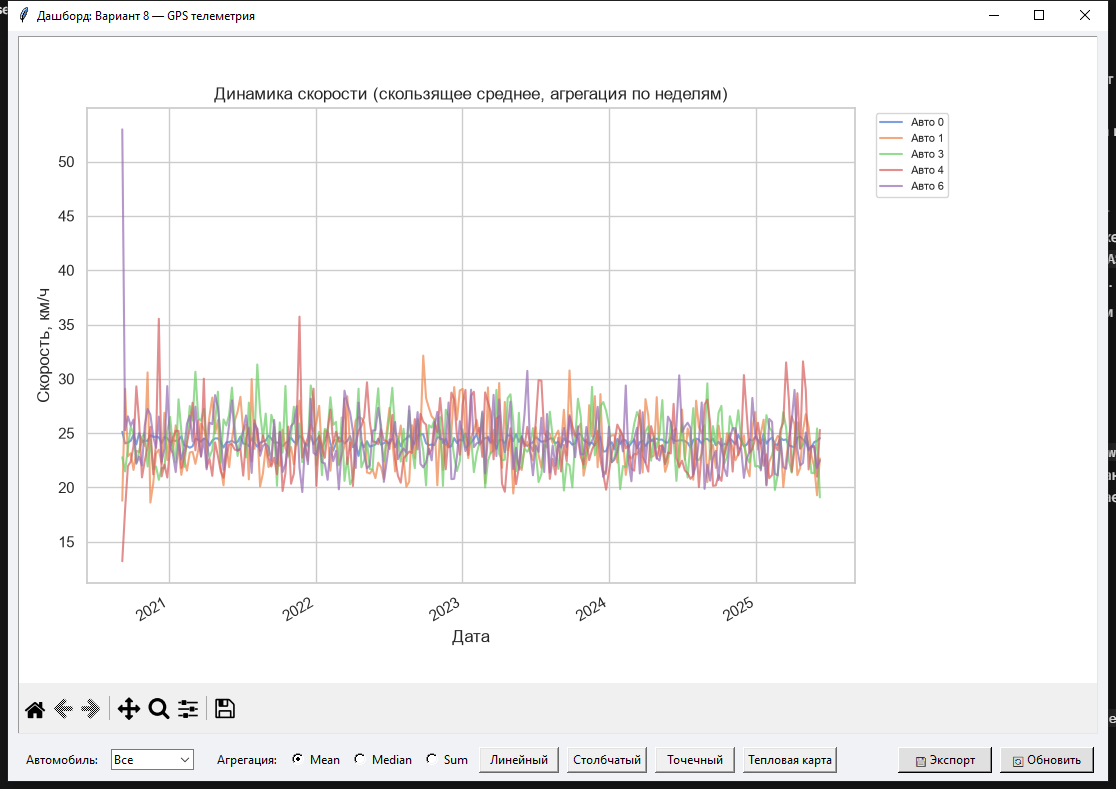
\includegraphics[width=\textwidth]{screenshots/01_line_all.png}
	\caption{Линейный график: динамика скользящей средней скорости по неделям (все автомобили)}
\end{figure}

\begin{figure}[H]
	\centering
	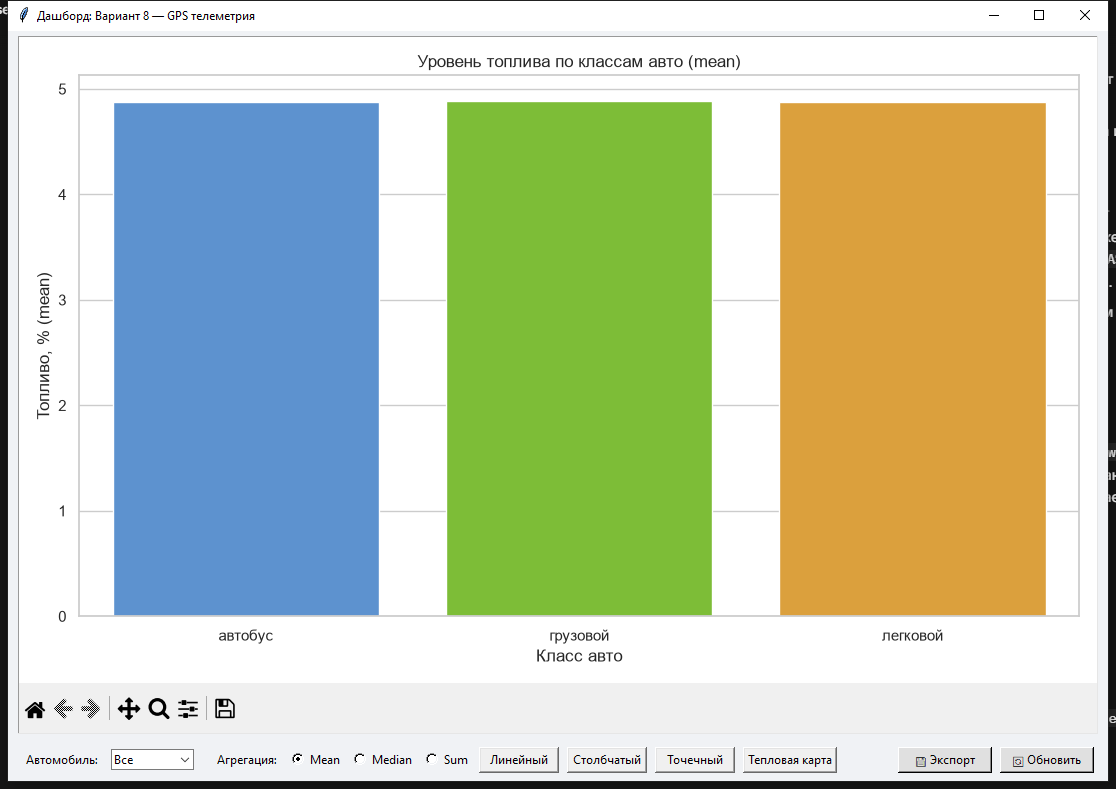
\includegraphics[width=\textwidth]{screenshots/03_bar_mean.png}
	\caption{Столбчатая диаграмма: уровень топлива по классам авто, агрегация \texttt{mean}}
\end{figure}

\begin{figure}[H]
	\centering
	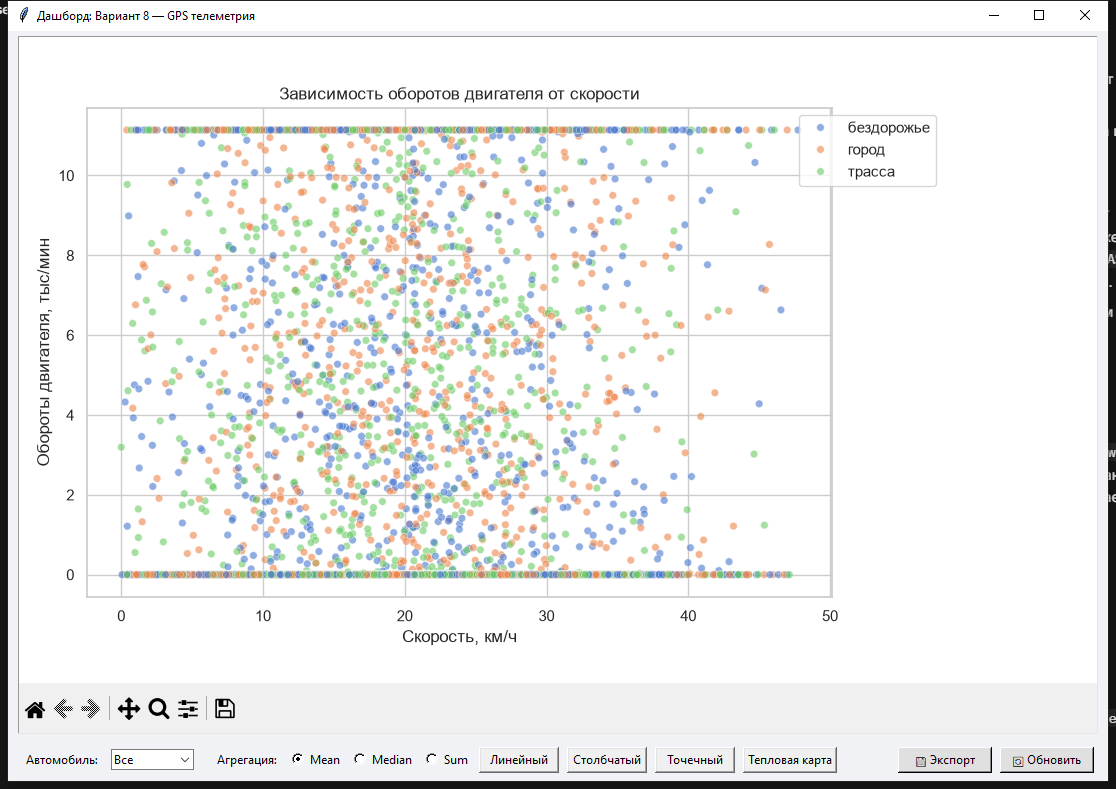
\includegraphics[width=\textwidth]{screenshots/05_scatter.png}
	\caption{Точечная диаграмма: зависимость оборотов двигателя от скорости с кодированием \texttt{road\_type}}
\end{figure}

\begin{figure}[H]
	\centering
	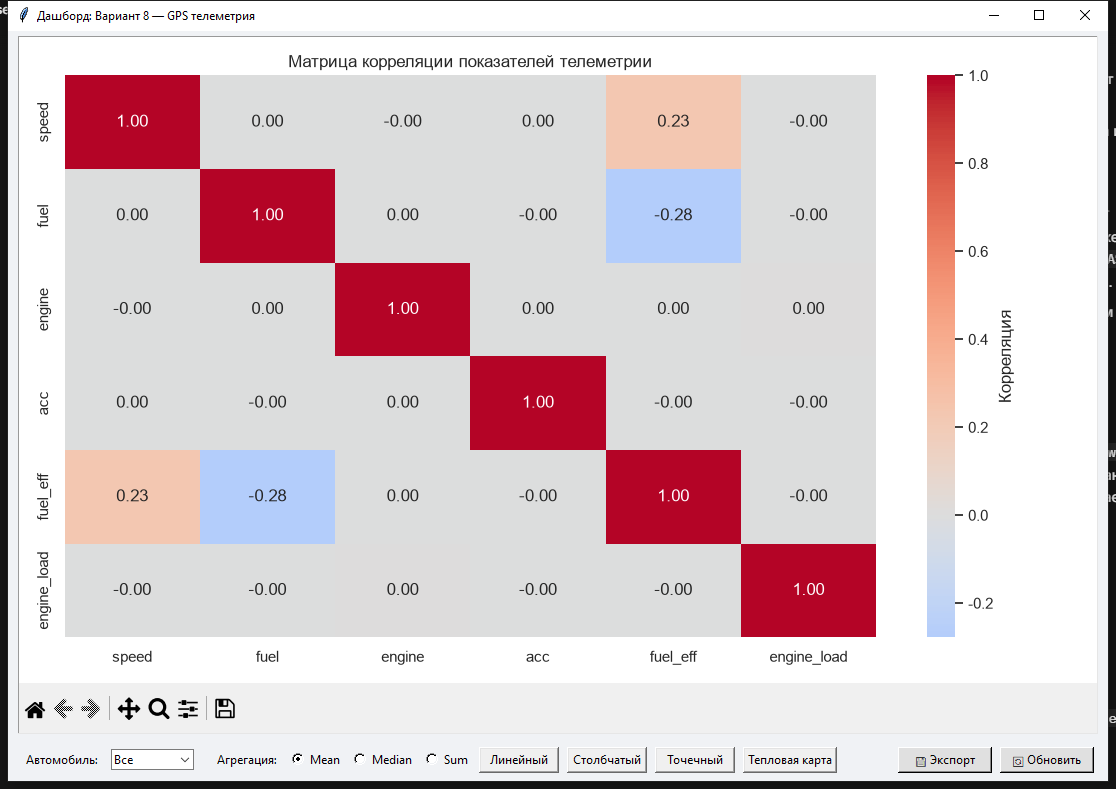
\includegraphics[width=\textwidth]{screenshots/06_heatmap.png}
	\caption{Тепловая карта корреляции числовых признаков телеметрии}
\end{figure}

\section{Анализ результатов}

В ходе выполнения лабораторной работы были получены следующие аналитические инсайты и выявлены системные ограничения. Основные количественные характеристики обработанного набора приведены в таблице~\ref{tab:lab7metrics}.

\begin{table}[H]
	\centering
	\caption{Метрики предобработки и работы дашборда}
	\label{tab:lab7metrics}
	\renewcommand{\arraystretch}{1.2}
	\begin{tabular}{|p{5.6cm}|p{3.2cm}|p{7.2cm}|}
		\hline
		Показатель & Значение & Комментарий \\
		\hline
		Исходных записей & 2\,000\,000 & Период 13.09.2020--15.06.2025, 249 недель \\
		\hline
		После фильтрации & 1\,755\,643 & Удалено 244\,357 записей (12,22\,\%) \\
		\hline
		Нефинитных значений & около 3\,\% & \texttt{speed} --- 59\,871, \texttt{fuel} --- 60\,260, \texttt{engine} --- 60\,209 \\
		\hline
		85-й перцентиль \texttt{engine} & 11,14 тыс/мин & Обрезано 263\,347 значений (15,00\,\%) \\
		\hline
		IQR-замены \texttt{speed} & 59\,653 (3,40\,\%) & Максимум 183,07 $\to$ 48,83 км/ч \\
		\hline
		Редкие \texttt{vehicle\_id} & 44 из 100 & 766\,988 записей объединены в категорию~0 \\
		\hline
		Категориальных признаков & 7 & 4 добавленных и 3 производных \\
		\hline
		Точек на точечной диаграмме & 5\,000 & Сэмплирование ради скорости отрисовки \\
		\hline
	\end{tabular}
\end{table}

Полученные инсайты:
\begin{itemize}[leftmargin=*]
	\item Исходный набор содержит 2\,000\,000 записей за период с 13.09.2020 по 15.06.2025 (249 недель). После удаления строк со \texttt{speed < 0} и \texttt{fuel > 100} осталось 1\,755\,643 записи (удалено 244\,357, или 12,22\,\%).
	\item Нефинитные значения присутствуют примерно в 3\,\% записей каждого вещественного поля: \texttt{speed} --- 59\,871, \texttt{fuel} --- 60\,260, \texttt{engine} --- 60\,209. Замена медианами до клаппинга предотвращает распространение \texttt{NaN} в производные признаки.
	\item 85-й перцентиль оборотов двигателя составил 11,14 тыс/мин; по нему обрезано 263\,347 значений (15,00\,\%). IQR-обработка по группам \texttt{vehicle\_id} заменила 59\,653 значения скорости (3,40\,\%), в результате чего максимальная скорость снизилась с 183,07 до 48,83 км/ч. Групповая обработка оказалась существенной: общая медиана «сгладила» бы индивидуальные особенности автомобилей.
	\item Скользящее среднее с окном $k=45$ эффективно сглаживает шум телеметрии. Распределение тренда почти симметрично: 877\,927 значений «разгон», 877\,616 --- «торможение», 100 --- «стабильно». Отсутствие заметного перекоса говорит об отсутствии систематического ускорения/торможения по автопарку, но высокая чувствительность знака разности к микроизменениям указывает на то, что признак тренда следует использовать вместе с порогом.
	\item Из 100 исходных \texttt{vehicle\_id} 44 категории встречаются реже порога в 17\,556 записей; в категорию~0 объединено 766\,988 записей (43,69\,\%), нередких идентификаторов осталось 55. Выпадающий список содержит только не редкие значения плюс категорию~0, что делает фильтрацию осмысленной.
	\item Добавлены четыре категориальных признака (\texttt{region}, \texttt{road\_type}, \texttt{weather}, \texttt{vehicle\_class}) и три производные категории (\texttt{speed\_category}, \texttt{season}, \texttt{speed\_trend}). Столбчатая диаграмма показывает почти одинаковый средний уровень топлива для всех классов авто (≈4,88\,\%), а медиана равна нулю из-за обилия отрицательных значений, обрезанных в ноль. Следовательно, признак \texttt{vehicle\_class}, сгенерированный независимо от телеметрии, не различает расход; для аналитики предпочтительнее группировка по \texttt{region} или \texttt{road\_type}.
	\item Точечная диаграмма и тепловая карта подтверждают практическое отсутствие линейной связи между скоростью и оборотами ($r \approx -0{,}0005$), скоростью и расходом ($r \approx 0{,}0003$), скоростью и флагом ускорения ($r \approx 0{,}0007$). Заметная отрицательная корреляция ($\approx -0{,}28$) между \texttt{fuel} и \texttt{fuel\_eff} является следствием деления на близкий к нулю уровень топлива: среднее \texttt{fuel\_eff} составляет $\approx 1{,}2 \cdot 10^{9}$. Этот производный признак требует дополнительной регуляризации знаменателя.
\end{itemize}

Выявленные ограничения:
\begin{itemize}[leftmargin=*]
	\item Архитектура Tkinter является однопоточной. При обработке 1,75 млн записей пересчёт \texttt{groupby()}, \texttt{rolling()} и отрисовка Seaborn могут вызывать кратковременные «фризы» интерфейса.
	\item Статический рендеринг Matplotlib/Seaborn не поддерживает аппаратное ускорение GPU, что ограничивает частоту обновления в режимах реального времени.
	\item Функция \texttt{canvas.draw\_idle()} ставит задачу в очередь событий, но не гарантирует мгновенного отражения данных при частых изменениях фильтров.
	\item Точечная диаграмма ограничена выборкой в 5000 записей ради скорости отрисовки, поэтому визуализация не отображает всю совокупность.
	\item Объединение 44 редких идентификаторов в категорию~0 создаёт крупную неоднородную группу; её статистики следует интерпретировать осторожно.
\end{itemize}

Пути масштабирования решения:
\begin{enumerate}[leftmargin=*]
	\item Перенос тяжёлых вычислений в фоновый поток с использованием \texttt{root.after()} или \texttt{queue.Queue} для безопасной передачи результатов в GUI-поток.
	\item Замена Seaborn на Plotly или Bokeh для нативной поддержки WebGL-ускорения и интерактивного масштабирования без потери производительности; для больших объёмов --- Datashader.
	\item Интеграция Dask DataFrame или Polars для распределённой обработки данных, выходящих за пределы RAM, с сохранением логики фильтрации на уровне API.
	\item Предварительная агрегация данных по неделям и категориям с кэшированием результата, а также вынесение параметра окна сглаживания в отдельный ползунок.
\end{enumerate}

\section{Выводы}

В ходе выполнения лабораторной работы были успешно освоены ключевые технологии создания интерактивных аналитических панелей в экосистеме Python:
\begin{itemize}[leftmargin=*]
	\item реализована событийно-ориентированная архитектура с использованием callback-функций и цикла событий \texttt{mainloop()}, что обеспечило мгновенный отклик интерфейса на действия пользователя;
	\item освоено встраивание графических объектов Matplotlib в оконную систему Tkinter через адаптер \texttt{FigureCanvasTkAgg}, включая корректную работу панели навигации \texttt{NavigationToolbar2Tk};
	\item на практике применены методы динамической фильтрации (\texttt{df.loc[]}, \texttt{df.query()}), агрегации (\texttt{groupby().agg()}), оконных функций (\texttt{rolling()}) и биннинга (\texttt{pd.cut()}) библиотеки pandas. Соблюдено правило обязательного копирования данных (\texttt{.copy()}) для предотвращения \texttt{SettingWithCopyWarning} и искажения исходного датасета;
	\item реализованы четыре типа интерактивных графиков и экспорт текущей визуализации в PNG/PDF;
	\item разработано устойчивое процедурное приложение без использования ООП-паттернов, что упростило отладку и чтение кода.
\end{itemize}

Трудности: основным вызовом стала синхронизация состояния данных между этапом предобработки и этапом отрисовки. Некорректное использование ссылок на DataFrame приводило к накоплению артефактов на графиках. Проблема была решена строгим разделением \texttt{df\_processed} (статический эталон) и \texttt{df\_work} (рабочая копия), а также использованием \texttt{fig.clear()} перед каждой отрисовкой. Дополнительная сложность была связана с нестабильностью производного признака \texttt{fuel\_eff} при малых значениях уровня топлива.

Пути улучшения: добавление логгирования событий, внедрение прогресс-баров для длительных вычислений, поддержка тёмной темы интерфейса, автоматическое сохранение состояния фильтров между сессиями и регуляризация знаменателей производных признаков.

\section{Ссылка на рабочую среду}

Исходный код дашборда находится в файле \texttt{main.py} папки \texttt{progalab 7}; исходные данные --- \texttt{data.csv}. Скриншоты работы программы сохранены в подпапке \texttt{screenshots}, экспортированные изображение и PDF --- в файлах \texttt{screenshots/exported\_plot.png} и \texttt{screenshots/exported\_plot.pdf}. Настоящий отчёт подготовлен в файле \texttt{report\_lab7.tex}, готовый PDF --- \texttt{report\_lab7.pdf}.

\end{document}
